\section{Phân tích Thiết kế hệ thống}

\subsection{User Stories của Game Player}
\subsection{User Stories}
\textbf{User Story về giao diện trò chơi:}
\begin{itemize}
	\item Là một Game Player, tôi muốn trò chơi chơi ở toàn màn hình.
	\item Là một Game Player, tôi muốn trò chơi chơi ở nhiều tỉ lệ khác nhau.
	\item Là một Game Player, tôi muốn menu có các nút đơn giản dễ sử dụng.
	\item Là một Game Player, tôi muốn giao diện trang bị trực quan, tôi có thể xem thông tin trang bị, cũng như sắp xếp và di chuyển trang bị từ khung trang bị vào kho đồ và ngược lại.
	\item Là một Game Player, tôi muốn giao diện bên ngoài màn chơi trực quan, các mục được hiện rõ ràng và dễ thao tác
	\item Là một Game Player, tôi muốn giao diện khi chiến đấu rõ ràng, các nút bấm dễ nhìn.
	\item Là một Game Player, tôi muốn giao diện bảng trả về trực quan, hiện đầy đủ thông tin, cũng như tôi có thể xem toàn bộ nội dung trong cell.
	\item Là một Game Player, tôi muốn player có thể hiển thị thông tin về tình trạng hiện tại, trang bị hiện có, những thông tin phải được cập nhật liên tục để tôi có thể xử lý các nước đi tiếp theo.
	\item Là một Game Player, tôi muốn có một hệ thống tab để tôi có thể chuyển đổi qua lại giữa các tab bảng trả về. 
	\item Là một Game Player, tôi muốn có hệ thống cài đặt cho phép cài đặt âm thanh, hình ảnh của trò chơi.
	\item Là một Game Player, tôi muốn có một phần để hiển thị thông tin của nhà phát triển.
	\item Là một Game Player, tôi muốn có một nút để thoát trò chơi.
	\item Là một Game Player, tôi muốn có nhiều người dùng được lưu trong game, mỗi người dùng sẽ có tên người chơi. Tôi có thể đổi được tên, thêm, xoá người dùng.
\end{itemize}
\textbf{User Story về cơ chế chơi:}
\begin{itemize}
	\item Là một Game Player, tôi muốn có nhiều màn chơi, chia thành nhiều Chapter để dễ theo dõi. Mỗi màn chơi sẽ hướng dẫn tôi những cơ chế mới của trò chơi với độ khó tăng dần.
	\item Là một Game Player, tôi muốn giao diện màn chơi đơn giản, dễ nhìn.
	\item Là một Game Player, tôi muốn trò chơi có phong cách đồ hoạ Fantasy, những nhân vật được nhân hoá.
	\item Là một Game Player, tôi muốn tôi có thể chèn, xoá, cập nhật các bảng trong schema tự do mà không bị lỗi.
	\item Là một Game Player, tôi muốn game có một sự phản hồi sau khi tôi nhập câu lệnh và chạy.
	\item Là một Game Player, tôi muốn player sẽ có một số phản ứng khi tôi nhập các câu lệnh nhất định (như attack hay use).
	\item Là một Game Player, tôi muốn trong màn chơi có hiển thị rõ các yêu cầu của màn chơi.
	\item Là một Game Player, tôi muốn sau khi bảng kết quả truy vấn hiện ra, tôi có thể xem toàn bộ nội dung của cell, sao chép nội dung đó hoặc sao chép toàn bộ hàng của bảng đó.
	\item Là một Game Player, tôi muốn có một nơi để tôi có thể ghi lại các ghi chú, gợi ý, hoặc dán nội dung đã sao chép từ bảng dữ liệu ra.
	\item Là một Game Player, tôi muốn có các animation cho các vật thể tương ứng với các hành động khác nhau, như idle, running, attacking,...
	\item Là một Game Player, trong trường hợp tôi nhập sai câu lệnh, hệ thống sẽ báo lỗi tôi sai như thế nào và tôi có thể chỉnh sửa lại câu lệnh sau cho đúng. 
	\item Là một Game Player, có thể chạy code ở cả chế độ chạy toàn bộ chương trình và chế độ debug (chạy từng dòng của chương trình).
	\item Là một Game Player, tôi muốn xem schema diagram, bản đồ của màn chơi.
	\item Là một Game Player, tôi muốn có một documentation về ngôn ngữ SQL và có một nút hiển thị để tôi có thể thuận tiện tra cứu.
	\item Là một Game Player, tôi muốn có một nút tạm dừng trò chơi, cũng như có thể save lại tiến trình màn chơi của tôi.
	\item Là một Game Player, tôi muốn tôi có thể chơi xuyên suốt toàn bộ màn chơi mà không gặp sự ngắt ngang bởi các yếu tố như quảng cáo,...
	\item Là một Game Player, sau khi hoàn thành màn chơi, tôi muốn một bảng hiện kết quả màn chơi kèm các nút bấm để di chuyển nhanh giữa các màn chơi.
\end{itemize}



\subsection{Các yêu cầu của hệ thống}
\subsubsection{Yêu cầu chức năng}
\subsubsection{Yêu cầu chức năng}
\textbf{Yêu cầu chức năng liên quan đến giao diện trò chơi:}
\begin{itemize}
	\item Trò chơi sẽ chơi ở chế độ toàn màn hình.
	\item Nhân vật chính xuất hiện ở màn chơi
	\item Giao diện trang bị trực quan, chia làm 3 phần: Kho đồ, slot trang bị và thông số người chơi. Có thể dùng chuột để xem thông tin trang bị, cũng như sắp xếp và di chuyển trang bị từ khung trang bị vào kho đồ và ngược lại.
	\item Giao diện bên ngoài màn chơi gồm bản đồ để chọn mà chơi. Thông tin màn chơi sẽ được hiện lên khi người chơi di chuột đến, cùng với các nút để mở giao diện trang bị và để vào shop để mua bán vật phẩm.
	\item Giao diện chơi được phân chia rõ ràng các khu vực, bao gồm vùng để chứa điều hướng Tab, thanh nhập câu lệnh, màn hình hiện kết quả trả về, vùng để chứa thông tin người chơi gồm 3 tab Stats, Equipments, Inventory, vùng chiến đấu và vùng giao diện phía trên chứa thông tin màn chơi và 4 nút Map, Schema, Docs, Settings để mở các hộp thoại tương ứng.
	\item Trong vùng chiến đấu, hiện rõ tên người chơi, tên quái vật và số bộ phần còn lại của quái vật.
	\item Khi gây sát thương, cần có dòng văn bản hiển thị số sát thương mà nhân vật tấn công gây ra cho đối phương. Sau khi kết thúc đòn đánh, có thể có một hộp thoại thông báo tính hiệu quả đòn đánh, xem đòn đánh có "Effective" hay không,...
	\item Có hộp thoại chứa schema diagram và bản đồ của màn chơi, giúp người chơi tra cứu.
	\item Có hộp thoại documentation về ngôn ngữ SQL để người chơi tham khảo.
	\item Vùng Player trên giao diện có thể hiển thị thông tin về tình trạng hiện tại, trang bị hiện có, những thông tin phải được cập nhật liên tục để người chơi có thể xử lý các nước đi tiếp theo.
	\item Giao diện bảng record trực quan, các cell dễ nhìn, có thể xem được toàn bộ nội dung cũng như có thể sao chép toàn bộ nội dung của cell, cũng như cũng có thể sao chép toàn bộ hàng. Ngoài ra Có một vùng để điều hướng sang các tab khác, mỗi tab là kết quả bảng trả về, ngoài ra còn có tab Notes cho người chơi ghi các ghi chú trong quá trình chơi.
	\item Menu của trò chơi gồm có các nút bấm: Play để bắt đầu chơi; Setting để người chơi thiết lập cài đặt trò chơi; Help để hiện giao diện hướng dẫn; Credit để hiển thị thông tin nhà phát hành; Exit để thoát trò chơi.
	\item Trò chơi có giao diện chuyển đổi người dùng, người chơi có thể thêm, xoá người dùng có phần để hiển thị tên của người chơi. Người chơi có thể tự do thay đổi tên.
\end{itemize}

\textbf{Yêu cầu chức năng liên quan đến cơ chế chơi:}
\begin{itemize}
	\item Chế độ cốt truyện được chia thành nhiều màn chơi, chia thành các Chapter cho mỗi khu vực lớn trên bản đồ. Mỗi màn chơi sẽ hướng dẫn tôi những cơ chế mới của trò chơi với độ khó tăng dần. Càng đi sâu trong màn chơi độ khó sẽ tăng dần. 
	\item Người chơi có thể chèn, xoá, cập nhật các bảng trong schema tự do mà không bị lỗi, trừ một số bảng đặc biệt. Đặc biệt là vùng chiến đấu, với các phản ứng của câu lệnh thì vùng chiến đấu sẽ có những hiển thị nhất định để cho người chơi thấy được những gì đã xảy ra sau khi người chơi chạy câu truy vấn.
	\item Các nhân vật có hoạt hình chuyển động, khi đang đợi lượt đi, khi tấn công, sử dụng vật phẩm, khi bị tấn công và khi bị tiêu diệt.
	\item Vùng chiến đấu hiển thị cấc thông tin về quái vật, về các phản ứng đòn đánh, về ngoại hình, hộp thoại cần được hiển thị chính xác để người chơi xác định đúng mục tiêu.
	\item Trong trường hợp người chơi nhập câu lệnh có lỗi ở mức SQL, hệ thống sẽ báo lỗi câu truy vấn sai như thế nào và sẽ không kết thúc lượt của người chơi, người chơi có thể chỉnh sửa lại sao cho đúng. 
	\item Cần có sự cân bằng trong game ở tất cả khía cạnh. Không thể để xảy ra trường hợp Over Powered (quá mạnh) hoặc Under Powered (quá yếu),...
	\item Cần xử lý các trường hợp người chơi cố tình thay đổi cấu trúc schema, chèn, update và xoá record trong bảng nhằm mục đích phá hoại, làm game bị lỗi và không thể hoạt động được nữa.
	\item Khi hoàn thành màn chơi, một bản thông báo sẽ xuất hiện. Bảng này hiển thị các thử thách đã đạt được và 3 nút bấm. Một nút bấm để trở về lựa chọn màn chơi, một nút bấm để chơi lại và một nút bấm để đến màn chơi kế tiếp.
	
\end{itemize}


\subsubsection{Yêu cầu phi chức năng}

\textbf{Yêu cầu phi chức năng liên quan đến Game Player:}
\begin{itemize}
	\item Hiệu năng ổn định, có thể chạy với 60FPS trong các ngữ cảnh khác nhau với cấu hình i5 - 8265U, Card Nvidia MX150, 12GB RAM. Có thể chạy với 120FPS khi tinh chỉnh cài đặt về đồ hoạ trên các cấu hình cao hơn.
	\item Giao diện của trò chơi nên đơn giản, dễ hiểu, phù hợp với nhiều loại người chơi. Cần tránh các thao tác rườm rà, phức tạp.
	Người chơi có thể thành thục chơi sau 30 phút trải nghiệm
	\item Phong cách đồ hoạ 2D Pixel, sử dụng các hiệu ứng kỹ xảo để đánh bóng game.
	\item Game giữ được sự ổn định khi quy mô của các object tăng lên, với nhiều object trong màn chơi ngày càng nhiều, hiệu ứng ngày càng dày đăc mà không có sự sụt giảm về hiệu năng.
	\item Game nên chạy mượt mà không gặp vấn đề lớn về bug, glitch. Hệ thống save load hoạt động hiệu quả, có thể lưu lại tiến trình màn chơi, kể cả khi tắt ngang trò chơi, hoặc sự cố về phần mềm như crash, sự cố về phần cứng và hệ điều hành.
	\item Các màn chơi cần có độ khó tăng dần, xoay tua giữa việc giới thiệu các tính năng mới và luyện tập các tính năng đã học. Màn chơi phải có độ khó vừa phải, không quá khó cũng không quá dễ.
	\item Thời gian phản ứng sau khi thực hiện câu truy vấn thấp, nhỏ hơn 1 giây. Sau khi chạy phải có kết quả trả về tương ứng với loại câu truy vấn.
\end{itemize}
\subsection{Usecase Diagram của Game}
\begin{figure}[H]
	\centering
	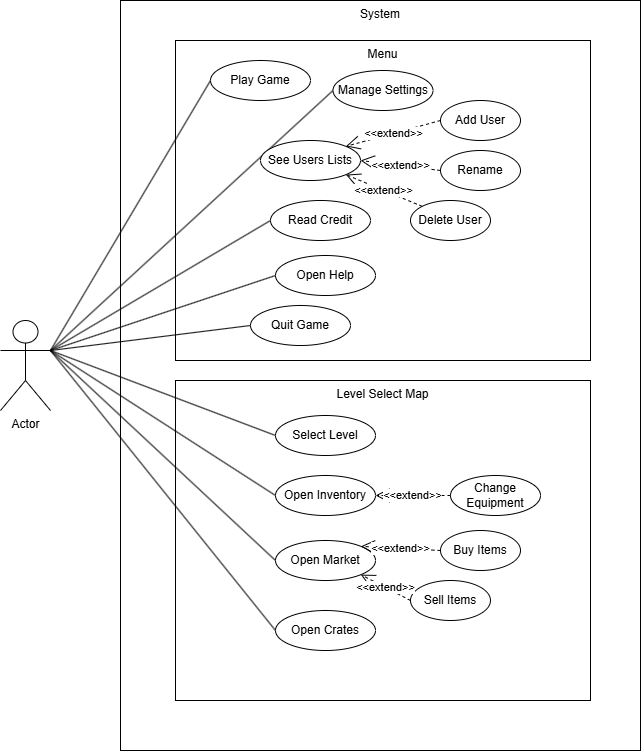
\includegraphics[width=\textwidth]{Images/UseCase.png}
	\vspace{0.5cm}
	\caption{Usecase Diagram của Game}
\end{figure}
\subsection{Một số Usecase tiêu biểu}
\subsubsection{Use case 1: Play game}
\begin{center}
	\begin{tabular}{|l|p{12cm}|}
		\hline
		ID and Name & UC1: Vào game \\
		\hline
		Actor  & Người chơi \\
		\hline
		Description  & Người chơi\\
		\hline
		Trigger  & Người chơi nhấn chuột trái vào nút Play.\\
		\hline
		Pre-conditions & \\
		\hline
		Post-conditions  & Màn hình Level Select Map hiện ra\\
		\hline
		\multirow{2}{*}{Normal flow}      &\qquad 1. Hệ thống lấy dữ liệu về màn chơi và profile hiện tại của người chơi.\\
		&\qquad 2. Hệ thống hiển thị màn hình chọn màn chơi\\
		\hline
		Alternative flow  & Người chơi lần đầu chơi -> hiện cutscene đầu game\\
		\hline
		Exceptions  &\\
		\hline
	\end{tabular}
\end{center}
\subsubsection{Use case 2: Add User}
\begin{center}
	\begin{tabular}{|l|p{12cm}|}
		\hline
		ID and Name & UC2: Add User \\
		\hline
		Actor  & Players \\
		\hline
		Description  & Người chơi \\
		\hline
		Trigger  & Người chơi ấn nút Create User\\
		\hline
		Pre-conditions & Người chơi đang sử dụng một tài khoản khác \\
		\hline
		Post-conditions  & Một người dùng đã được tạo ra.\\
		\hline
		\multirow{2}{*}{Normal flow}      &\qquad 1. Hộp thoại nhập tên người dùng được hiện lên\\
		&\qquad 2. Người dùng nhập tên người dùng và ấn OK\\
		&\qquad 3. Hệ thống tạo thành công người dùng mới và chuyển quyền truy cập hiện tại sang người chơi mới\\
		\hline
		Alternative flow  & Tên người dùng đã có -> hệ thống yêu cầu người dùng nhập tên mới\\
		\hline
		Exceptions  & Không thể lưu dữ liệu do không thể ghi vào tệp cần thiết\\
		\hline
	\end{tabular}
\end{center}
\subsubsection{Use case 3: Rename User}
\begin{center}
	\begin{tabular}{|l|p{12cm}|}
		\hline
		ID and Name & UC3: Rename User \\
		\hline
		Actor  & Players \\
		\hline
		Description  & Người chơi đổi tên người dùng hiện tại hoặc tên một người dùng khác\\
		\hline
		Trigger  & Người chơi nhận chuột trái vào tên user trong danh sách và nhấn nút Rename\\
		\hline
		Pre-conditions & Người chơi đang có ít nhất một người dùng trong game \\
		\hline
		Post-conditions  & Tên người dùng đã được đổi.\\
		\hline
		\multirow{2}{*}{Normal flow}      &\qquad 1. Hộp thoại Rename hiện lên\\
		&\qquad 2. Người dùng nhập tên người dùng mới và ấn OK\\
		&\qquad 3. Hệ thống đổi tên thành công người dùng\\
		\hline
		Alternative flow  & Tên người dùng đã có -> hệ thống yêu cầu người dùng nhập tên mới\\
		\hline
		Exceptions  & Không thể lưu dữ liệu do không thể ghi vào tệp cần thiết\\
		\hline
	\end{tabular}
\end{center}
\subsubsection{Use case 4: Delete User}
\begin{center}
	\begin{tabular}{|l|p{12cm}|}
		\hline
		ID and Name & UC4: Delete User \\
		\hline
		Actor  & Players \\
		\hline
		Description  & Người chơi xoá người dùng khi không muốn sử dụng người dùng đó nữa\\
		\hline
		Trigger  & Người chơi nhận chuột trái vào tên user trong danh sách và nhấn nút Delete\\
		\hline
		Pre-conditions & Người chơi đang có ít nhất một người dùng trong game \\
		\hline
		Post-conditions  & Người dùng chỉ định đã được xoá, nếu người dùng bị xoá là người dùng hiện tại, chuyển truy cập game sang người dùng khác. Nếu không còn người dùng nào nữa, hiện hộp thoại Create User.\\
		\hline
		\multirow{2}{*}{Normal flow}      &\qquad 1. Hộp thoại xác nhận Delete hiện lên\\
		&\qquad 2. Người dùng ấn OK\\
		&\qquad 3. Hệ thống xoá thành công người dùng\\
		\hline
		Alternative flow  & Người dùng nhấn Cancel trong hộp thoại xác nhận, quá trình bị huỷ bỏ\\
		\hline
		Exceptions  & Không thể lưu dữ liệu do không thể ghi vào tệp cần thiết\\
		\hline
	\end{tabular}
\end{center}
\subsubsection{Use case 5: Switch User}
\begin{center}
	\begin{tabular}{|l|p{12cm}|}
		\hline
		ID and Name & UC5: Switch User \\
		\hline
		Actor  & Players \\
		\hline
		Description  & Người chơi chuyển đổi quyền truy cập game sang người dùng khác\\
		\hline
		Trigger  & Người chơi nhấn chuột trái vào nút Switch User\\
		\hline
		Pre-conditions & \\
		\hline
		Post-conditions  & Người dùng được chuyển sang một người dùng được chỉ định\\
		\hline
		\multirow{2}{*}{Normal flow}      &\qquad 1. Hộp thoại danh sách người dùng được hiện lên, đi kèm với tiến trình và các thông tin sơ bộ được hiện lên. \\
		&\qquad 2. Người dùng chọn người dùng muốn chuyển sang và ấn Switch, hoặc đúp chuột vào người dùng muốn chuyển\\
		&\qquad 3. Hệ thống chuyển sang người dùng được chỉ định và đưa người chơi về màn hình menu chính\\
		\hline
		Alternative flow  & Người dùng nhấn Cancel trong hộp thoại xác nhận, quá trình bị huỷ bỏ\\
		\hline
		Exceptions  & Không thể load dữ liệu do file lưu bị lỗi\\
		\hline
	\end{tabular}
\end{center}
\subsubsection{Use case 6: Select Level}
\begin{center}
	\begin{tabular}{|l|p{12cm}|}
		\hline
		ID and Name & UC6: Select Level \\
		\hline
		Actor  & Players \\
		\hline
		Description  & Người chơi chọn level muốn chơi\\
		\hline
		Trigger  & Người chơi nhấn chuột trái vào nút Play Game và đợi quá trình loading hoàn tất\\
		\hline
		Pre-conditions & Người chơi đã hoàn thành màn chơi tutorial\\
		\hline
		Post-conditions  & Màn chơi được chọn được load và hiên trên màn hình, người chơi bắt đầu màn chơi.\\
		\hline
		\multirow{2}{*}{Normal flow}      &\qquad 1. Màn hình bản đồ chọn level hiện lên, gồm nhiều level trải dài trên các vùng trên bản đồ.\\
		&\qquad 2. Người dùng di chuyển chuột đến nút chọn level, một hộp thoại hiển thị thông tin sơ bộ của màn chơi, với sơ lược màn chơi, thử thách và cấp độ cần thiết của người chơi, cũng như level có chơi được không.\\
		&\qquad 3. Người chơi click vào nút chọn màn chơi.\\
		&\qquad 4. Hệ thống load màn chơi được chỉ định, nếu tồn tại tiến trình màn chơi được chỉ định thì sẽ load luôn tiến trình màn chơi, không thì sẽ load màn chơi và bắt đầu từ đầu màn chơi\\
		\hline
		Alternative flow  & Màn chơi không có sẵn hoặc bị khoá. Người dùng chọn một màn chơi khác\\
		\hline
		Exceptions  & Game bị crash, dữ liệu màn chơi không hợp lệ hoặc dữ liệu tiến trình của người chơi bị lỗi.\\
		\hline
	\end{tabular}
\end{center}
\subsubsection{Use case 7: Change Equipment}
\begin{center}
	\begin{tabular}{|l|p{12cm}|}
		\hline
		ID and Name & UC7: Change Equipment \\
		\hline
		Actor  & Players \\
		\hline
		Description  & Người chơi đưa trang bị từ Inventory và ngược lại. Người chơi sắp xếp, hoán đổi vị trí trang bị trang bị...\\
		\hline
		Trigger  & Người chơi nhấn chuột trái vào nút Inventory và màn hình Inventory hiện ra\\
		\hline
		Pre-conditions &\\
		\hline
		Post-conditions  & Người chơi hoán đổi vị trí trang bị thành công.\\
		\hline
		\multirow{2}{*}{Normal flow}      &\qquad 1. Trên màn hình Equipment và Inventory, người chơi dùng chuột kéo thả món trang bị mình muốn đến ô như mong muốn. Ô mong muốn có thể là ô trang bị cũng như ô trong inventory\\
		&\qquad 2. Nếu ô được chỉ định không hợp lệ, item được trả về vị trí cũ. Nếu hợp lệ, đưa item đến ô chỉ định\\
		&\qquad 3. Nếu ô chỉ định có item, tráo đổi vị trí hai item với nhau. Nếu item không phải là trang bị được trỏ đến ô trang bị, trả về vị trí cũ\\
		&\qquad 4. Cập nhật các thông số mới nếu có sự thay đổi về trang bị.\\
		\hline
		Alternative flow  & Nếu cấp độ người chơi không đủ để trang bị món trang bị, người dùng chọn một vật phẩm khác\\
		\hline
		Exceptions  & Game bị crash, dữ liệu màn chơi không hợp lệ.\\
		\hline
	\end{tabular}
\end{center}